% qibao1/qibao1.tex —— 七宝中学高一上周末作业 1（试卷版/答案版）
% 试卷版：xelatex qibao1.tex
% 答案版：xelatex "\def\isanswer{1}\input{qibao1.tex}"

\documentclass[a4paper,11pt]{article}
\usepackage{common}

\begin{document}

\examtitlest{2026--2027 学年度七宝中学高一上周末作业 1}{集合与常用逻辑用语}

\bigsec{一、填空题}

\begin{enumerate}
\setcounter{enumi}{2}

\item 设 $A=\{x\mid x^2-3x+2=0\}$，$B=\{x\mid ax-2=0\}$，且 $B\subseteq A$，则实数 $a$ 组成的集合是 \blankline[2em].

\ans{$\{0,1,2\}$}

\ifanswer
\solbegin
\step{由 $x^2-3x+2=0$，解得 $x=1$ 或 $2$，故 $A=\{1,2\}$，由 $B\subseteq A$，故分两种情况：当 $B=\varnothing$ 时，即 $a=0$ 时，满足题意；}
\step{当 $B\neq\varnothing$ 时，即 $a\neq 0$ 时，$B=\{\tfrac{2}{a}\}$，故 $\tfrac{2}{a}=1$ 或 $\tfrac{2}{a}=2$，解得 $a=2$ 或 $a=1$.}
\step{综上所述，实数 $a$ 组成的集合为 $\{0,1,2\}$.}
\solend

\fi
\item 已知 $M\cup\{1,2\}=\{1,2,3\}$，则集合 $M$ 所有可能的个数是 \blankline 个.

\ans{$4$}

\ifanswer
\solbegin
\step{$M$ 可能情况有 $\{3\}$、$\{1,3\}$、$\{2,3\}$、$\{1,2,3\}$，故集合 $M$ 所有可能的个数是 4 个.}
\solend

\fi
\item 若集合 $\{0,-1,2a\}=\{a-1,-|a|,a+1\}$，实数 $a$ 的值为 \blankline[2em].

\ans{$\pm 1$}

\ifanswer
\solbegin
\step{令 $A=\{0,-1,2a\}$，$B=\{a-1,-|a|,a+1\}$.}
\step{因为 $\{0,-1,2a\}=\{a-1,-|a|,a+1\}$，若 $a-1=0$，则 $a=1$，则 $A=\{0,-1,2\}$，$B=\{0,-1,2\}$，满足要求；}
\step{若 $-|a|=0$，则 $a=0$，则 $A=\{0,-1,0\}$，不满足集合元素的互异性；}
\step{若 $a+1=0$，则 $a=-1$，则 $A=\{0,-1,-2\}$，$B=\{0,-1,-2\}$，满足要求.}
\step{故实数 $a$ 的值为 $\pm 1$.}
\solend

\fi
\item 已知集合 $A=\{x\mid x^2+2x-8=0\}$，$B=\{x\mid x^2-5x+6=0\}$，$C=\{x\mid x^2-mx+m^2-13=0\}$，若 $B\cap C\neq\varnothing$，$A\cap C=\varnothing$，则 $m=$ \blankline[2em].

\ans{$4$}

\ifanswer
\solbegin
\step{$A=\{x\mid x^2+2x-8=0\}=\{-4,2\}$，$B=\{x\mid x^2-5x+6=0\}=\{2,3\}$.}
% 注：原卷此句作「所以 $3\in C$，$2\notin C$，$-4\notin C$」；本稿曾把 $2\notin C$ 写成 $2\in C$
%     （与题干 $A\cap C=\varnothing$ 及 $2\in A$ 直接矛盾），2026-09-15 回原图核对时已订正。
\step{因为 $B\cap C\neq\varnothing$，$A\cap C=\varnothing$，所以 $3\in C,\,2\notin C,\,-4\notin C$.}
\step{由 $3\in C$ 得 $9-3m+m^2-13=0$，即 $m^2-3m-4=0$，解得 $m=-1$ 或 $m=4$.}
\step{当 $m=-1$ 时，解 $x^2+x-12=0$ 得 $C=\{-4,3\}$，此时 $A\cap C=\{-4\}$，不满足题意.}
\step{当 $m=4$ 时，解 $x^2-4x+3=0$ 得 $C=\{1,3\}$，满足题意.}
\step{所以 $m=4$.}
\solend

\fi
\item 已知集合 $A=\{x\mid -1\leqslant x+1\leqslant 6\}$，$B=\{x\mid m-1<x<2m+1,\,m\in\R\}$，若 $A\cup B=A$，则实数 $m$ 的取值范围为 \blankline[2em].

\ans{$(-\infty,-2]\cup[-1,2]$}

\ifanswer
\solbegin
\step{$A=\{x\mid -1\leqslant x+1\leqslant 6\}=\{x\mid -2\leqslant x\leqslant 5\}$.}
\step{当 $m-1\geqslant 2m+1$，即 $m\leqslant -2$ 时，$B=\varnothing$ 满足 $B\subseteq A$.}
\step{当 $m-1<2m+1$，即 $m>-2$ 时，要使 $B\subseteq A$ 成立，需 $\begin{cases}m-1\geqslant -2 \\ 2m+1\leqslant 5\end{cases}$，得 $-1\leqslant m\leqslant 2$.}
\step{综上，实数 $m$ 的取值范围为 $(-\infty,-2]\cup[-1,2]$.}
\solend

\fi
\item 已知集合 $M=\left\{x\mid x=\tfrac{m}{n},\,n\in\mathbb{N},\,x\in\mathbb{N}\right\}$ ($1\leqslant m\leqslant 10,\,m\in\mathbb{N}$) 共有 8 个子集，则 $m$ 的取值集合为 \blankline[2em].

\ans{$\{4,9\}$}

\ifanswer
\solbegin
\step{集合 $M=\left\{x\mid x=\tfrac{m}{n},\,n\in\mathbb{N},\,x\in\mathbb{N}\right\}$ ($1\leqslant m\leqslant 10,\,m\in\mathbb{N}$) 中有 8 个子集，由 $2^3=8$ 得集合 $M$ 中有三个元素，则 $m$ 有三个因数，因为 $x=\tfrac{m}{n}$，$n\in\mathbb{N}^*$，$1\leqslant m\leqslant 10$，$m\in\mathbb{N}^*$，所以除 1 和它本身 $m$ 外，还有 1 个.}
\step{所以 $m$ 的取值集合为 $\{4,9\}$.}
\solend

\fi
\item 设集合 $A=\{x\mid 1\leqslant x\leqslant 10,\,x\in\mathbb{N}\}$，$B=\{y\mid y=x^2-12x+36,\,x\in A\}$，则集合 $A\cap B=$ \blankline[2em].

\ans{$\{1,4,9\}$}

\ifanswer
\solbegin
\step{集合 $A=\{x\mid 1\leqslant x\leqslant 10,\,x\in\mathbb{N}\}=\{1,2,3,4,5,6,7,8,9,10\}$，$B=\{y\mid y=x^2-12x+36,\,x\in A\}=\{25,16,9,4,1,0\}$，所以集合 $A\cap B=\{1,4,9\}$.}
\solend

\fi
\item 已知集合 $A=\{x\mid x\geqslant 4\text{ 或 }x<-5\}$，$B=\{x\mid a+1\leqslant x\leqslant a+3\}$，若 $B\subseteq A$，则实数 $a$ 的取值范围 \blankline[2em].

\ans{$\{a\mid a<-8\text{ 或 }a\geqslant 3\}$}

\ifanswer
\solbegin
\step{若 $B\subseteq A$，则 $a+3<-5$ 或 $a+1\geqslant 4$，解得 $a<-8$ 或 $a\geqslant 3$.}
\solend

\fi
% 注：原卷题干作「若规定集合 $E=\{0,1,2,\cdots,n\}$ 的子集 $\{a_1,a_2,a_3,\cdots,a_m\}$ 为 $E$ 的第 $k$ 个子集」
%     （原卷此处上标用 $n$、子集下标用 $m$，并不统一）；本稿曾把上标也写成 $m$，
%     2026-09-15 回原图核对时按原卷改回 $n$。
% 又：原卷【解析】与【答案】作「$211=2^7+2^6+2^4+2^1+2^0$，则 $E$ 的第 211 个子集是 $\{0,1,4,6,7\}$」；
%     本稿曾把指数写成 $2^2$（那样和为 213）、答案漏掉 7（作 $\{0,1,4,6\}$，仅 83），同日一并订正。
\item 若规定集合 $E=\{0,1,2,\dots,n\}$ 的子集 $\{a_1,a_2,a_3,\dots,a_m\}$ 为 $E$ 的第 $k$ 个子集，其中 $k=2^{a_1}+2^{a_2}+2^{a_3}+\dots+2^{a_m}$，则 $E$ 的第 211 个子集是 \blankline[2em].

\ans{$\{0,1,4,6,7\}$}

\ifanswer
\solbegin
\step{用 2 的幂从大到小依次表示 211 即可，$211=2^7+2^6+2^4+2^1+2^0$，则 $E$ 的第 211 个子集是 $\{0,1,4,6,7\}$.}
\solend

\fi
\item 已知非空集合 $A,B$ 满足以下三个条件：

① $A\cup B=\{1,2,3,4,5,6,7\}$，$A\cap B=\varnothing$；

② $A$ 的元素个数不是 $A$ 中的元素，$B$ 的元素个数不是 $B$ 中的元素；

③ $A$ 中所有元素之和为偶数（若 $A$ 为单元集，则该元素为偶数）.

则有序集合对 $(A,B)$ 的个数为 \blankline 个.

\ans{$16$}

\ifanswer
\solbegin
\step{由条件①得，集合 $A$、$B$ 中的元素个数之和为 7.}
\stepm{(1)}{若集合 $A$ 中只有 1 个元素，$B$ 中有 6 个元素，由条件②得 $1\notin A,\,6\notin B$，则 $6\in A$，$1\in B$.}
\step{再由条件①得 $A=\{6\}$，$B=\{1,2,3,4,5,7\}$，此时满足条件③.}
\step{此时有 1 种情形.}
\stepm{(2)}{若集合 $A$ 中有 2 个元素，$B$ 中有 5 个元素，由条件②得 $2\notin A,\,5\notin B$，得 $5\in A$，$2\in B$.}
\step{若满足条件③中所有元素之和为偶数（若 $A$ 为单元集，则该元素为偶数），当 $A=\{1,5\}$ 时，$B=\{2,3,4,6,7\}$；}
\step{当 $A=\{3,5\}$ 时，$B=\{1,2,4,6,7\}$；}
\step{当 $A=\{5,7\}$ 时，$B=\{1,2,3,4,6\}$，此时有 3 种情形.}
\stepm{(3)}{若集合 $A$ 中有 3 个元素，$B$ 中有 4 个元素，由条件②得 $3\notin A,\,4\notin B$，得 $4\in A$，$3\in B$.}
\step{若满足条件③中所有元素之和为偶数（若 $A$ 为单元集，则该元素为偶数），当 $A=\{1,4,5\}$ 时，$B=\{2,3,6,7\}$；}
\step{当 $A=\{1,4,7\}$ 时，$B=\{2,3,5,6\}$；}
\step{当 $A=\{4,5,7\}$ 时，$B=\{1,2,3,6\}$；}
\step{当 $A=\{2,4,6\}$ 时，$B=\{1,3,5,7\}$，此时有 4 种情形.}
\stepm{(4)}{若集合 $A$ 中有 4 个元素，$B$ 中有 3 个元素，由条件②得 $4\notin A,\,3\notin B$，得 $3\in A$，$4\in B$.}
\step{若满足条件③中所有元素之和为偶数（若 $A$ 为单元集，则该元素为偶数），当 $A=\{1,2,3,6\}$ 时，$B=\{4,5,7\}$；}
\step{当 $A=\{2,3,5,6\}$ 时，$B=\{1,4,7\}$；}
\step{当 $A=\{2,3,6,7\}$ 时，$B=\{1,4,5\}$；}
\step{当 $A=\{1,3,5,7\}$ 时，$B=\{2,4,6\}$，此时有 4 种情形.}
\stepm{(5)}{若集合 $A$ 中有 5 个元素，$B$ 中有 2 个元素，由条件②得 $5\notin A,\,2\notin B$，得 $2\in A$，$5\in B$.}
\step{若满足条件③中所有元素之和为偶数（若 $A$ 为单元集，则该元素为偶数），当 $A=\{2,3,4,6,7\}$ 时，$B=\{1,5\}$；}
\step{当 $A=\{1,2,4,6,7\}$ 时，$B=\{3,5\}$；}
\step{当 $A=\{1,2,3,4,6\}$ 时，$B=\{5,7\}$，此时有 3 种情形.}
\stepm{(6)}{若集合 $A$ 中有 6 个元素，$B$ 中有 1 个元素，由条件②得 $6\notin A,\,1\notin B$，得 $1\in A$，$6\in B$.}
\step{所以 $A=\{1,2,3,4,5,7\}$，$B=\{6\}$，满足条件③.}
\step{此时有 1 种情形.}
\step{综上所述，有序集合对 $(A,B)$ 的个数为 $1+3+4+4+3+1=16$ 个.}
\solend

\fi
\end{enumerate}

\bigsec{二、选择题}

\begin{enumerate}
\setcounter{enumi}{12}

\item 已知集合 $M=\{0,1,2\}$，$N=\{x\mid x=2a,\,a\in M\}$，$M\cup N=$（\quad）.

A. $N$\qquad B. $M$\qquad C. $\{0,2,4\}$\qquad D. $\{0,1,2,4\}$

\ans{D}

\item 如果 $a^{2025}+b^{2025}=0$，那么一定有（\quad）.

A. $(|a|+|b|)^{2025}=0$\qquad B. $(a-b)^{2025}=0$\qquad C. $(a\cdot b)^{2025}=0$\qquad D. $(a+b)^{2025}=0$

\ans{D}

\ifanswer
\solbegin
\step{由 $a^{2025}+b^{2025}=0$，得 $a^{2025}=-b^{2025}=(-b)^{2025}$，则 $(a^{2025})^{\tfrac{1}{2025}}=[(-b)^{2025}]^{\tfrac{1}{2025}}$，即 $a=-b$，即 $a+b=0$.}
\step{故 $(a+b)^{2025}=0$，故 D 符合题意.}
\step{对于 A，若取 $a=1,\,b=-1$，则 $(|a|+|b|)^{2025}=2^{2025}\neq 0$，故 A 不合题意.}
\step{对于 B，若取 $a=1,\,b=-1$，则 $(a-b)^{2025}=2^{2025}\neq 0$，故 B 不合题意.}
\step{对于 C，若取 $a=1,\,b=-1$，则 $(a\cdot b)^{2025}=(-1)^{2025}=-1\neq 0$，故 C 不合题意.}
\step{故选 D.}
\solend

\fi

% 注：原卷此题印有一张韦恩图（矩形全集 $I$，$M$、$P$ 两圆相交、$S$ 为含于 $P$ 的小圆，
%     阴影为 $(M\cap P)\setminus S$）；本稿此前漏排此图而题干仍作「如图」，
%     2026-09-15 回原图核对时按原图补入。
% 注：本题题干、韦恩图与选项须排在同一页，故在图前加 \filbreak（放不下就整块移到下一页）。
\filbreak
\item 如图，$I$ 为全集，$M$、$P$、$S$ 是 $I$ 的三个子集，则阴影部分所表示的集合是（\quad）.

\begin{center}
% 插图取自原卷截图（裁去截图残影后 4× LANCZOS 放大），不用 TikZ 手绘
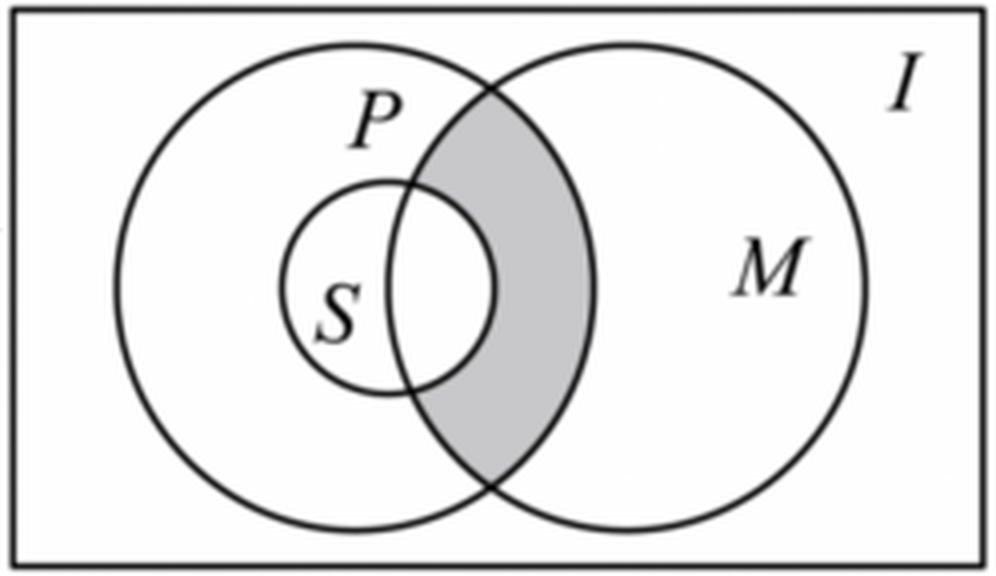
\includegraphics[width=0.40\textwidth]{figures/venn_MP_minus_S.png}
\end{center}

A. $(M\cap P)\cap S$\qquad B. $(M\cap P)\cup S$\qquad C. $(M\cap P)\cap\overline{S}$\qquad D. $(M\cap P)\cup\overline{S}$

\ans{C}

\ifanswer
\solbegin
\step{由 Venn 图得，集合表示 $M$、$P$ 的交集与 $S$ 的补集的交集，即阴影部分所表示的集合是 $(M\cap P)\cap\overline{S}$，故选 C.}
\solend

\fi

\item 定义一种集合运算 $nand$ 为：$A\,\text{nand}\,B=\{x\mid x\notin A\text{ 或 }x\notin B\}$，设全集为 $U$，给定集合 $A$ 与 $B$，则仅使用 $nand$ 运算和 $A,B,U$，①可以表示 $A\cup B$；②可以表示 $A\cap B$，则下列说法正确的是（\quad）.

A. ① 正确，② 错误\qquad B. ①② 都正确\qquad C. ①② 都错误\qquad D. ① 错误，② 正确

\ans{B}

\ifanswer
\solbegin
\step{由题意得集合运算 $nand$ 为 $A$ 与 $B$ 的补集的并集，由于 $U$ 的补集是空集，所以 $U\,\text{nand}\,A=\overline{A}$，进一步有 $(U\,\text{nand}\,A)\,\text{nand}\,(U\,\text{nand}\,B)=\overline{A}\,\text{nand}\,\overline{B}=A\cup B$.}
\step{$U\,\text{nand}\,(A\,\text{nand}\,B)=A\cap B$，故选 B.}
\solend

\fi
\end{enumerate}

\bigsec{三、解答题}

\begin{enumerate}
\setcounter{enumi}{16}

\item 设集合 $P=(-2,3)$，$Q=\{x\mid 3a<x\leqslant a+1\}$.
\begin{enumerate}[label=(\arabic*)]
\item 若 $Q\subseteq P$，求实数 $a$ 的取值范围；
\item 若 $P\cap Q=\varnothing$，求实数 $a$ 的取值范围.
\end{enumerate}

\ans{（1）$\left[-\tfrac{2}{3},+\infty\right)$；（2）$(-\infty,-3]\cup\left[\tfrac{1}{2},+\infty\right)$}

\ifanswer
\solbegin
\stepm{(1)}{当 $Q=\varnothing$ 时，$3a\geqslant a+1$，解得 $a\geqslant\tfrac{1}{2}$，满足题意.}
% 注：原卷此处的方程组含三行「$\begin{cases}3a\geqslant -2 \\ a+1<3 \\ 3a<a+1\end{cases}$」（末行即 $Q\neq\varnothing$ 本身）；
%     本稿曾略去末行、只留两行，2026-09-15 回原图核对时按原卷补回。
\step{当 $Q\neq\varnothing$ 时，因为 $Q\subseteq P$，所以 $\begin{cases}3a\geqslant -2 \\ a+1<3 \\ 3a<a+1\end{cases}$，解得 $-\tfrac{2}{3}\leqslant a<\tfrac{1}{2}$.}
\step{综上所述，实数 $a$ 的取值范围为 $\left[-\tfrac{2}{3},+\infty\right)$.}
\stepm{(2)}{当 $Q=\varnothing$ 时，$3a\geqslant a+1$，解得 $a\geqslant\tfrac{1}{2}$，满足题意.}
\step{当 $Q\neq\varnothing$ 时，因为 $P\cap Q=\varnothing$，所以 $\begin{cases}a+1\leqslant -2 \\ 3a<a+1\end{cases}$ 或 $\begin{cases}3a\geqslant 3 \\ 3a<a+1\end{cases}$，解得 $a\leqslant -3$ 或 无解.}
\step{综上所述，实数 $a$ 的取值范围为 $(-\infty,-3]\cup\left[\tfrac{1}{2},+\infty\right)$.}
\solend

\fi
\ansspace[6]
\item 已知集合 $A=\{x\mid x^2+4x=0\}$，$B=\{x\mid x^2+2(a+1)x+a^2-1=0\}$.
\begin{enumerate}[label=(\arabic*)]
\item 若 $A$ 是 $B$ 的子集，求实数 $a$ 的值；
\item 若 $B$ 是 $A$ 的子集，求实数 $a$ 的取值范围.
\end{enumerate}

\ans{（1）$a=1$；（2）$(-\infty,-1]\cup\{1\}$}

\ifanswer
\solbegin
\stepm{(1)}{因为 $A=\{-4,0\}$，$B=\{x\mid x^2+2(a+1)x+a^2-1=0\}$，又 $A\subseteq B$，所以 $A=B$，所以 $\begin{cases}-4+0=-2(a+1) \\ -4\times 0=a^2-1\end{cases}$，所以 $a=1$.}
\stepm{(2)}{因为 $B$ 是 $A$ 的子集，所以 $B=\varnothing$ 或 $B=\{-4\}$ 或 $B=\{0\}$ 或 $B=\{-4,0\}$.}
\stepm{①}{$B=\varnothing$ 时，$\Delta=4(a+1)^2-4(a^2-1)<0$，所以 $a<-1$.}
\stepm{②}{$B=\{-4\}$ 时，$\begin{cases}-4+(-4)=-2(a+1) \\ -4\times(-4)=a^2-1\end{cases}$，无解.}
\stepm{③}{$B=\{0\}$ 时，$\begin{cases}0+0=-2(a+1) \\ 0\times 0=a^2-1\end{cases}$，所以 $a=-1$.}
\stepm{④}{$B=\{-4,0\}$ 时，由 (1) 得 $a=1$.}
\step{综上，实数 $a$ 的取值范围为 $(-\infty,-1]\cup\{1\}$.}
\solend

\fi
\ansspace[6]
\item 已知集合 $A=\{x\mid -3<2x+1<7\}$，$B=\{x\mid x<-4\text{ 或 }x>2\}$，$C=\{x\mid 3a-2<x<a+1\}$.
\begin{enumerate}[label=(\arabic*)]
\item 求 $A\cap\overline{B}$；
\item 若“$p:x\in\overline{A\cup B}$”是“$q:x\in C$”的充分不必要条件，求实数 $a$ 的取值范围.
\end{enumerate}

\ans{（1）$\{x\mid -2<x\leqslant 2\}$；（2）$\left(-3,-\tfrac{2}{3}\right)$}

\ifanswer
\solbegin
\stepm{(1)}{因为 $A=\{x\mid -3<2x+1<7\}=\{x\mid -2<x<3\}$，又 $\overline{B}=\{x\mid -4\leqslant x\leqslant 2\}$，所以 $A\cap\overline{B}=\{x\mid -2<x\leqslant 2\}$.}
\stepm{(2)}{$A\cup B=\{x\mid x<-4\text{ 或 }x>-2\}$，所以 $\overline{A\cup B}=\{x\mid -4\leqslant x\leqslant -2\}$.}
\step{因为“$p:x\in\overline{A\cup B}$”是“$q:x\in C$”的充分不必要条件，所以 $\overline{A\cup B}\subseteq C$，又 $C=\{x\mid 3a-2<x<a+1\}$.}
\step{所以 $\begin{cases}3a-2<-4 \\ a+1>-2\end{cases}$，得 $-3<a<-\tfrac{2}{3}$.}
\step{故实数 $a$ 的取值范围是 $\left(-3,-\tfrac{2}{3}\right)$.}
\solend

\fi
\ansspace[7]
\item 设非空集合 $S$ 具有如下性质：① 元素都是正整数；② 若 $x\in S$，则 $10-x\in S$.
\begin{enumerate}[label=(\arabic*)]
\item 请你写出符合条件的，且分别含有一个、二个、三个元素的集合 $S$ 各一个；
\item 是否存在恰有 6 个元素的集合 $S$？若存在，写出所有的集合 $S$；若不存在，请说明理由；
\item 满足条件的集合 $S$ 总共有多少个？
\end{enumerate}

\ans{（1）一个：$\{5\}$；二个：$\{1,9\}$（不唯一）；三个：$\{1,5,9\}$（不唯一）；（2）存在，4 个；（3）31 个}

\ifanswer
\solbegin
\stepm{(1)}{一个：$\{5\}$；}
\step{二个：$\{1,9\}$（不唯一）；}
\step{三个：$\{1,5,9\}$（不唯一）.}
\stepm{(2)}{存在，一共有四个，$S=\{1,2,3,7,8,9\}$ 或 $S=\{1,2,4,6,8,9\}$ 或 $S=\{1,3,4,6,7,9\}$ 或 $S=\{2,3,4,6,7,8\}$.}
\stepm{(3)}{$S\subseteq\{1,2,3,4,5,6,7,8,9\}$.}
\step{含有一个元素的集合 $S$ 有 1 个：$\{5\}$.}
\step{含有两个元素的集合 $S$ 有 4 个：$\{1,9\},\allowbreak\{2,8\},\allowbreak\{3,7\},\allowbreak\{4,6\}$.}
\step{含有三个元素的集合 $S$ 有 4 个：$\{1,5,9\},\allowbreak\{2,5,8\},\allowbreak\{3,5,7\},\allowbreak\{4,5,6\}$.}
\step{含有四个元素的集合 $S$ 有 6 个：$\{1,9,2,8\},\allowbreak\{1,9,3,7\},\allowbreak\{1,9,4,6\},\allowbreak\{2,8,3,7\},\allowbreak\{2,8,4,6\},\allowbreak\{3,7,4,6\}$.}
\step{含有五个元素的集合 $S$ 有 6 个：$\{1,9,5,2,8\},\allowbreak\{1,9,5,3,7\},\allowbreak\{1,9,5,4,6\}$，$\{2,8,5,3,7\},\allowbreak\{2,8,5,4,6\},\allowbreak\{3,7,5,4,6\}$.}
\step{含有六个元素的集合 $S$ 有 4 个：$\{1,9,2,8,3,7\},\allowbreak\{1,9,2,8,4,6\},\allowbreak \\
\{1,9,3,7,4,6\},\allowbreak\{2,8,3,7,4,6\}$.}
\step{含有七个元素的集合 $S$ 有 4 个：$\{1,9,2,5,8,3,7\},\allowbreak\{1,9,2,5,8,4,6\},\allowbreak\{1,9,5,3,7,4,6\},\allowbreak\{2,8,3,5,7,4,6\}$.}
\step{含有八个元素的集合 $S$ 有 1 个：$\{1,2,3,4,6,7,8,9\}$.}
\step{含有九个元素的集合 $S$ 有 1 个：$\{1,2,3,4,5,6,7,8,9\}$.}
\step{所以符合条件的 $S$ 共有 $1+4+4+6+6+4+4+1+1=31$ 个.}
\solend

\fi
\ansspace[8]
\ansneed{7cm}
\item 若集合 $A$ 具有以下性质，则称集合 $A$ 是“好集”：① $0\in A$，$1\in A$；② 若 $x$、$y\in A$，则 $x-y\in A$，且 $x\neq 0$ 时，$\tfrac{1}{x}\in A$.
\begin{enumerate}[label=(\arabic*)]
\item 分别判断集合 $B=\{-1,0,1\}$、有理数集 $Q$ 是否是“好集”，并说明理由；
\item 设集合 $A$ 是“好集”，求证：若 $x$、$y\in A$，则 $x+y\in A$；
\item 对任意的一个“好集”$A$，判断下面命题的真假，并说明理由：命题：若 $x$、$y\in A$，则必有 $xy\in A$.
\end{enumerate}

\ans{（1）$B$ 不是“好集”，$Q$ 是“好集”；（2）略；（3）真}

\ifanswer
\solbegin
\stepm{(1)}{集合 $B$ 不是“好集”，理由是：$-1\in B$，$1\in B$，而 $-1-1=-2\notin B$；}
\step{所以 $B$ 不是“好集”.}
\step{有理数集 $Q$ 是“好集”，理由是：$0\in Q$，$1\in Q$；}
\step{对任意 $x\in Q$，$y\in Q$，有 $x-y\in Q$，且 $x\neq 0$ 时，$\tfrac{1}{x}\in Q$；}
\step{所以有理数集 $Q$ 是“好集”.}
\stepm{(2)}{因为集合 $A$ 是“好集”，所以 $0\in A$.}
\step{若 $x$、$y\in A$，则 $0-y\in A$，即 $-y\in A$，所以 $x-(-y)\in A$，即 $x+y\in A$.}
\stepm{(3)}{对任意一个“好集”$A$，任取 $x$、$y\in A$.}
\step{若 $x$、$y$ 中有 0 和 1 时，显然 $xy\in A$.}
\step{下设 $x$、$y$ 均不含 $0$、$1$，由定义得 $x-1$、$\tfrac{1}{x-1}$、$\tfrac{1}{x}\in A$.}
\step{所以 $\tfrac{1}{x-1}-\tfrac{1}{x}=\tfrac{1}{x(x-1)}\in A$，所以 $x(x-1)\in A$.}
\step{由 (2) 得 $x(x-1)+x=x^2\in A$，同理 $y^2\in A$.}
\step{若 $x+y=0$ 或 $x+y=1$，显然 $(x+y)^2\in A$.}
\step{若 $x+y\neq 0$ 且 $x+y\neq 1$，则 $(x+y)^2\in A$.}
\step{得 $2xy=(x+y)^2-x^2-y^2\in A$，所以 $\tfrac{1}{2xy}\in A$.}
\step{由 (2) 得 $\tfrac{1}{xy}=\tfrac{1}{2xy}+\tfrac{1}{2xy}\in A$，所以 $xy\in A$.}
\step{综上，$xy\in A$.}
\solend

\fi
\ansspace*[9]
\end{enumerate}

\end{document}